\section{Strumenti}
\begin{wrapfigure}{r}{100mm}
    \centering
    \begin{subfigure}[h]{0.3\textwidth}
        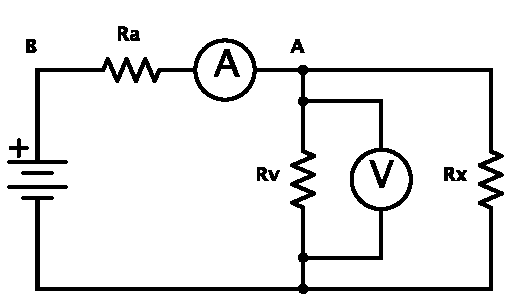
\includegraphics[width=\textwidth]{R_monte.pdf}
        \caption{Schema del cricuito con amperometro a monte}
        \label{fig:monte}
    \end{subfigure}%
    ~ %add desired spacing between images, e. g. ~, \quad, \qquad etc.
      %(or a blank line to force the subfigure onto a new line)
    \begin{subfigure}[h]{0.3\textwidth}
        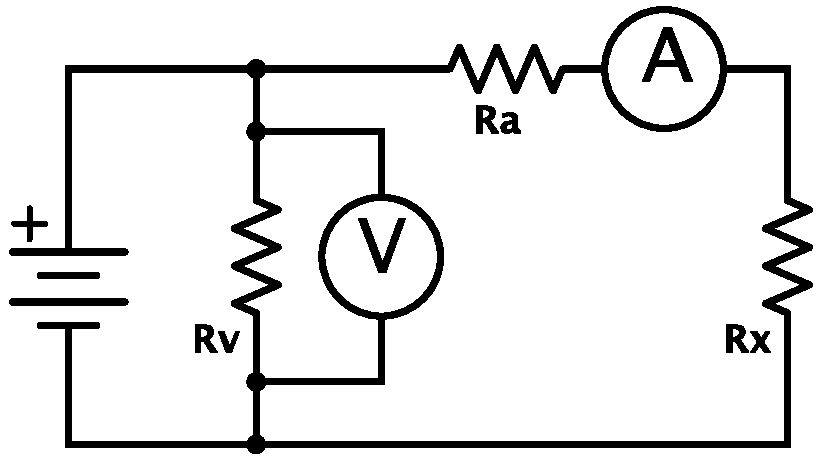
\includegraphics[width=\textwidth]{R_valle.pdf}
        \caption{Schema del cricuito con amperometro a valle}
        \label{fig:valle}
    \end{subfigure}%
    \caption{blah blah blah}
    \label{fig:circuiti}
\end{wrapfigure}


$\quad \bullet \quad$7 resistenze:\\
$\quad \quad$1, 10, 100, 1k, 10k, 100k, 1M$\Omega$\\
$\quad \bullet \quad$Cablaggio\\
$\quad \bullet \quad$2 tester ICE\\
$\quad \bullet \quad$Generatore di corrente DC\\
$\quad \bullet \quad$Multimetro digitale\\
$\quad \bullet \quad$Breadboard o basetta sperimentale\\

% è da finire!!!